\title{Homework 3 Report}
\author{
        Hooley Cheng \\
                Department of Mathematics\\
        University of Washington\\
        Seattle, WA, 98105, U.S.
           
}
\date{\today}

\documentclass[12pt]{article}


\usepackage{amsmath}
\usepackage{graphicx}
\usepackage{float}
\usepackage{listings}

\usepackage{titlesec}
\begin{document}
\maketitle

\begin{abstract}
This project intends to explore various properties of principal component analysis, PCA. The data we used is obtained by extracting the track of an paint can hanged with a spring.
\end{abstract}

\section{Introduction and Overview}\
	Principal Component Analysis is a very useful tool that helps us analysing data an reduce redundancy. In order to get deep understanding of real-world data, we need to find a method to get rid of all kinds of noise. Therefore, In this project, we are going to use various method to achieve that goal, including PCA. And we will locate the can from 12 different videos.\\
	
	There are 3 groups videos captured by different position, and, in each group, there are 4 different videos captured under different condition: ideal, noisy, horizontal displacement and rotation. 
	
\section{Theoretical Background}
\subsection{Singular Value Decomposition}
SVD de-composites a Matrix $A$ in to three components $U, S, V$. and
\[A = USV\]
where $U$  is an $ m\times m$ real or complex unitary matrix, $S$ is an $ m\times n$ rectangular diagonal matrix with non-negative real numbers on the diagonal, and$V$ is a $ n\times n$ real or complex unitary matrix.
One of properties of $S$ is that if there are redundancy in our data, then there will only have several large numbers, with the rest of the singular values being very close to 0.
\subsection{Principal Component Analysis}
The key to analysing a given experiment is to consider the covariance matrix
\[C_X = \frac{1}{n - 1}X*X^T\]
And SVD gives us a very easy approach to get this matrix. SVD can diagonalize any matrix by working in the appropriate pair of bases $U$ and $V$. Thus by defining the transformed variable
\[Y=U*X\]
where$X = USV$. Then:
\begin{align*}
C_Y &= \frac{1}{n-1}YY^T\\
&= \frac{1}{n-1}(U^*X)(U^*X)^T\\
&= \frac{1}{n-1}U^*(UU^T)U \\
&= \frac{1}{n-1} U^*US^2UU^*\\
C_Y &= \frac{1}{n - 1}S^2
\end{align*}
\section{Algorithm Implementation and Development}
We first need to extract the movement of the object, and we could clearly see that the brightness of the can is much higher than any other places. Therefore, we could design a kernel and use convolution to found the region that has max brightness. Also, the size of the kernel defines the size of our window scanner, so we could use this data to get the position of the moving objects. Then, we could perform SVD on our data to see if there is anything special to notice.
\section{Computational Results}
\subsection{Ideal Case}
\begin{figure}[H]
\begin{tabular}{cc}
  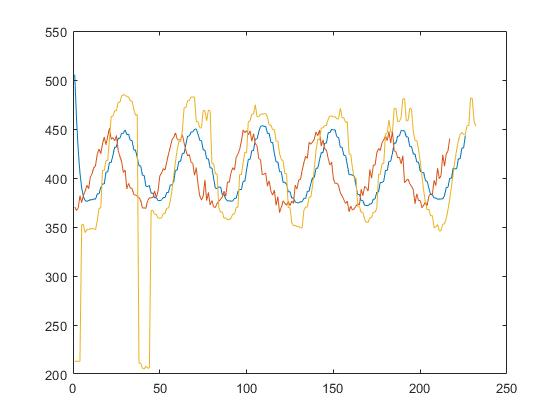
\includegraphics[width=\textwidth]{N_1.jpg}
\end{tabular}
\end{figure}
From this figure, we can clearly see that three cameras recorded approximately the same oscillatory movement.
\begin{figure}[H]
\begin{tabular}{cc}
  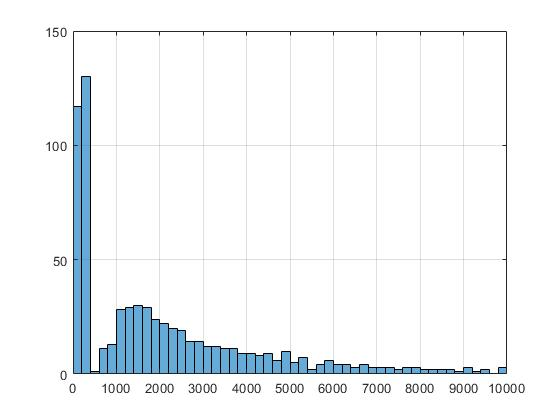
\includegraphics[width=\textwidth]{N_1_variance.jpg}
\end{tabular}
\end{figure}
From this figure, we can see that most singular values are less than 5000, and only a few exceeded than that boundary.
\subsection{Noisy Case}
\begin{figure}[H]
\begin{tabular}{cc}
  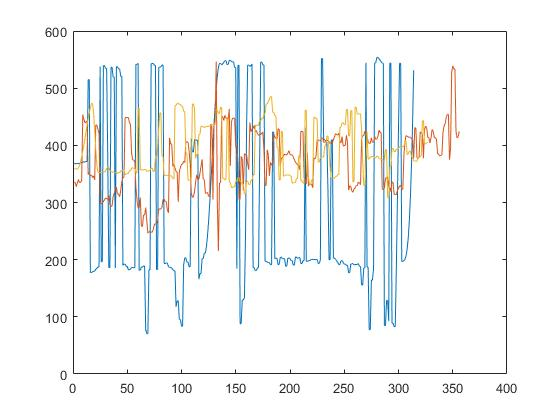
\includegraphics[width=\textwidth]{N_2.jpg}
\end{tabular}
\end{figure}
It is very hard to tell what kind of movement it is from this noisy data, but we can still see that there are some patterns that implies it is oscillation, Thought it is nearly impossible to extract properties of this.
\begin{figure}[H]
\begin{tabular}{cc}
  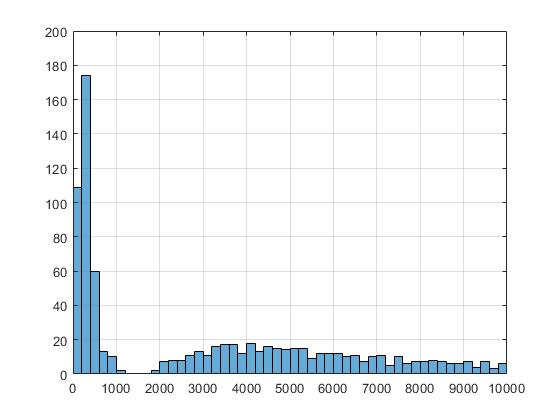
\includegraphics[width=\textwidth]{N_2_variance.jpg}
\end{tabular}
\end{figure}
From this figure, we can see that most singular values are less than 1500, and only a few exceeded than that boundary.
\subsection{Horizontal displacement}
\begin{figure}[H]
\begin{tabular}{cc}
  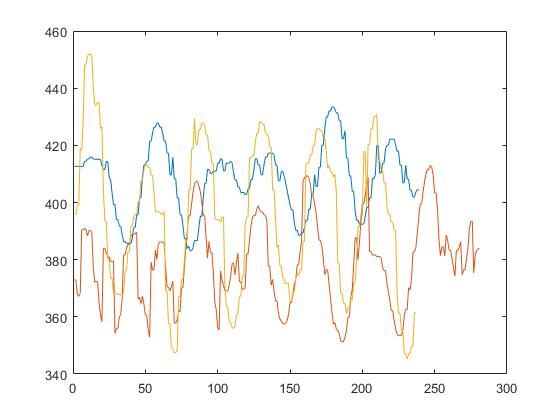
\includegraphics[width=\textwidth]{N_3.jpg}
\end{tabular}
\end{figure}
Again, this figure clearly shows the oscillatory pattern of this objects, and three movements are approximately the same.
\begin{figure}[H]
\begin{tabular}{cc}
  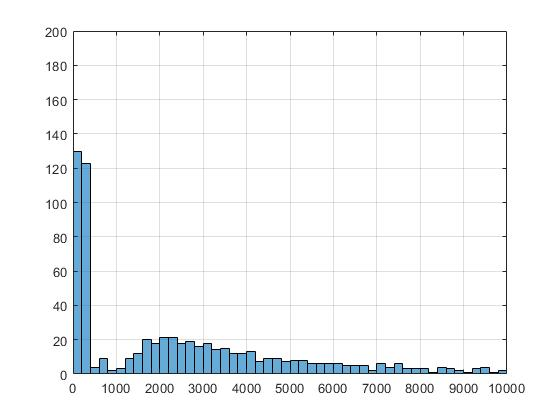
\includegraphics[width=\textwidth]{N_3_variance.jpg}
\end{tabular}
\end{figure}
From this figure, we can see that most singular values are less than 1000, and only a few exceeded than that boundary.
\subsection{ Horizontal displacement and rotation}
\begin{figure}[H]
\begin{tabular}{cc}
  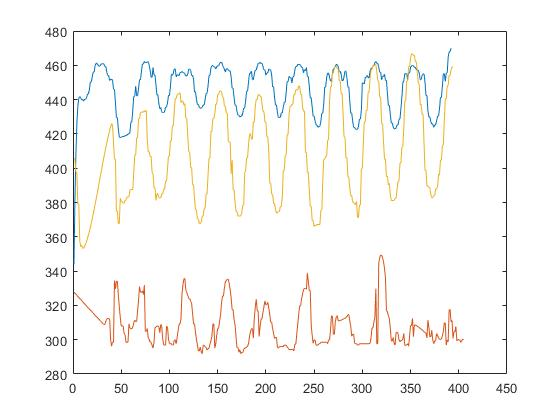
\includegraphics[width=\textwidth]{N_4.jpg}
\end{tabular}
\end{figure}
\begin{figure}[H]
\begin{tabular}{cc}
  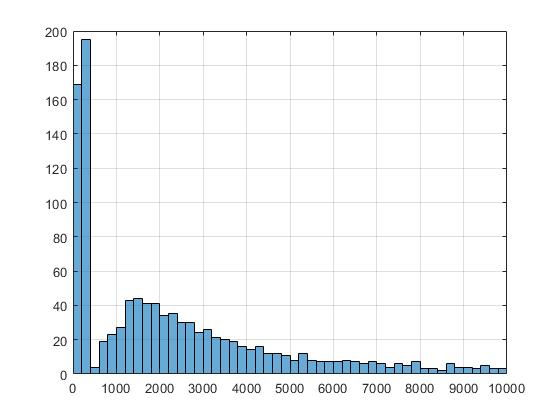
\includegraphics[width=\textwidth]{N_4_variance.jpg}
\end{tabular}
\end{figure}
From this figure, we can see that most singular values are less than 5000, and only a few exceeded than that boundary.
\section{Summary and Conclusions}
In this project, We used SVD and PCA to reduce redundancy from our data. Also, We found that noise does have a great negative impact on our analysis and final outcomes, which is showed in case 2.
\section{Appendix A}
s = svd(A) returns the singular values of matrix A in descending order.\\
C = conv2(A,B) returns the two-dimensional convolution of matrices A and B.
\section{Appendix B: Matlab Source Code}
section{MATLAB codes}
\begin{verbatim}
function [displacement, X] = findpath(data, on)
    numFrames1_1 = size(data, 4);
    %Y = uint8(zeros(480, 640, 226));
    X = zeros( 480 * 640, 226);

    for j = 1:numFrames1_1
        i = data(:,:,:,j);
        gray = rgb2gray(i);
        X(:, j) = reshape(gray,[1, 480 * 640]);
end

for i = 1:480*640
    X(i, :) = X(i, :) - mean(X(i, :));
end
width = 70;
height = 100;
figure(1)
P1 = zeros(2, numFrames1_1);
for j = 1:numFrames1_1
    image = reshape(X(:,j),[480, 640]);
    kernel = ones(height, width);
    pimage = abs(image);
    pimage(1:160,1:680) = 0;
    output = conv2(kernel, pimage);
    maxval = max(output(:));
    [y, x] = find(output == maxval);
    y = y - height;
    x = x - width; 
    P1(:, j) = [y, x];
    if on == 1
        subplot(2,2,1) 
        imagesc(image);
        axis equal
        hold on
        rectangle('Position',[x,y,width, height],'Edgecolor', 'r');
        hold off
        drawnow
        subplot(2,2,2)
        i = data(:,:,:,j);
        imshow(i);
        hold on
        rectangle('Position',[x,y,width, height],'Edgecolor', 'r');
        hold off
        drawnow
    end
end
displacement = sqrt(P1(1,:).^2 + P1(2,:).^2);
displacement = filloutliers(displacement,'makima');
if on == 1
    figure(3)
    plot(1:length(displacement), displacement);
end
end

[d1_1, X1_1] = findpath(vidFrames1_4, 0);
[d2_1, X2_1] = findpath(vidFrames2_4, 0);
[d3_1, X3_1] = findpath(vidFrames3_4, 0);
[u1,s1,v1] = svd(X1_1, 'econ');
[u2,s2,v2] = svd(X2_1, 'econ');
[u3,s3,v3] = svd(X3_1, 'econ');
from = 0;
end1 = 10000;
lambda = [diag(s1);diag(s2);diag(s3)];
figure(6)
edges = linspace(0, end1, 51)
histogram(lambda, 'BinEdges',edges); axis([from end1 0 200])
grid on;
xlim([from, end1]);
\end{verbatim}
\end{document}